\chapter{Dinámica Temporal y Análisis de Supervivencia}

En este capítulo se abandona la visión estática de las cohortes para profundizar en la evolución temporal de los estudiantes. Utilizando técnicas de análisis de supervivencia, se estima la probabilidad real de egreso corrigiendo el sesgo de censura informativa identificado previamente.

\section{Estimación de Kaplan-Meier por Licenciatura}

La Figura \ref{fig:supervivencia_global} muestra la probabilidad de permanecer sin titularse en función del tiempo activo. Se observa una diferencia estructural entre ambas carreras: mientras que en Física la mediana de egreso se sitúa en los 17.0 semestres (con un intervalo de confianza al 95\% de $[16.0, 18.0]$), en Matemáticas más del 50\% de la población no alcanza la titulación dentro del periodo de observación de 20 semestres (mediana y límite superior indefinidos).

Para confirmar que esta divergencia no es producto del azar, se aplicó una prueba estadística Log-Rank. Los resultados arrojaron un estadístico de prueba de $\chi^2 = 5.85$ y un p-valor de $p \approx 0.0156$. Al ser $p < 0.05$, se concluye rigurosamente que existe una diferencia estadísticamente significativa en las probabilidades de supervivencia académica entre Matemáticas y Física.

\begin{figure}[H]
    \centering
    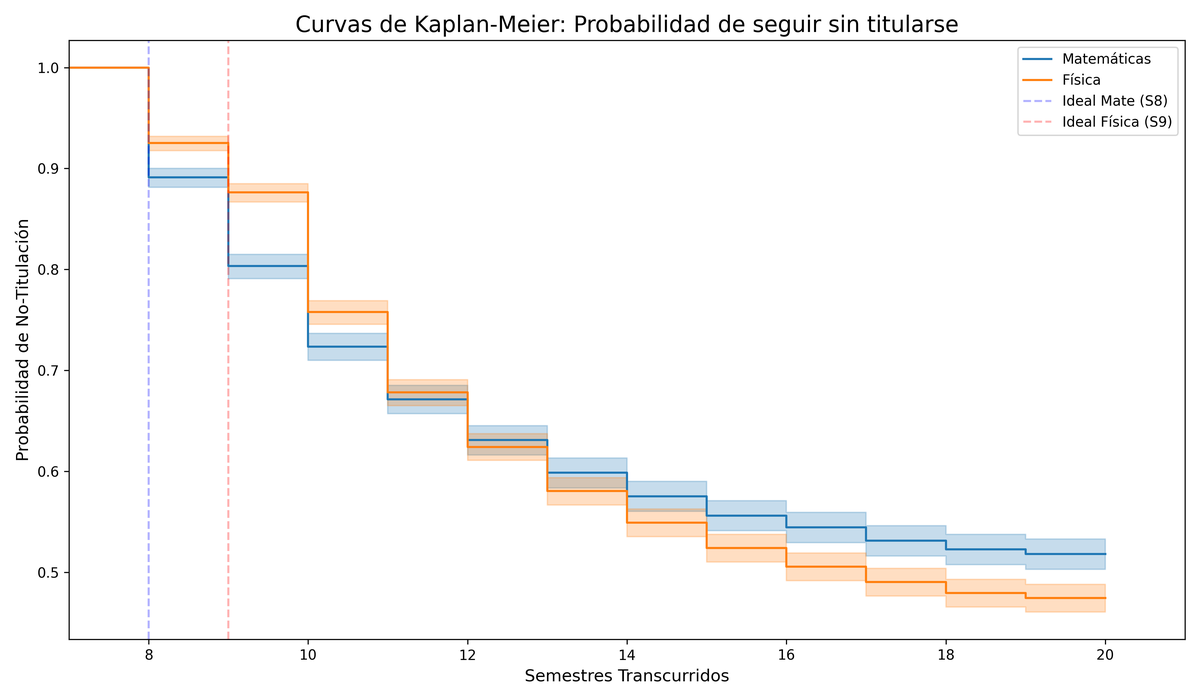
\includegraphics[width=0.8\textwidth]{imagenes/supervivencia_global.png}
    \caption{Curvas de supervivencia global para Matemáticas y Física. Las líneas punteadas indican los tiempos ideales de egreso (S8 y S9).}
    \label{fig:supervivencia_global}
\end{figure}

\section{Trayectorias y Perfiles de Egreso}

Para entender el origen de estas diferencias, se analizaron las trayectorias secuenciales del promedio real en contraste con las curvas de supervivencia.

\begin{figure}[H]
    \centering
    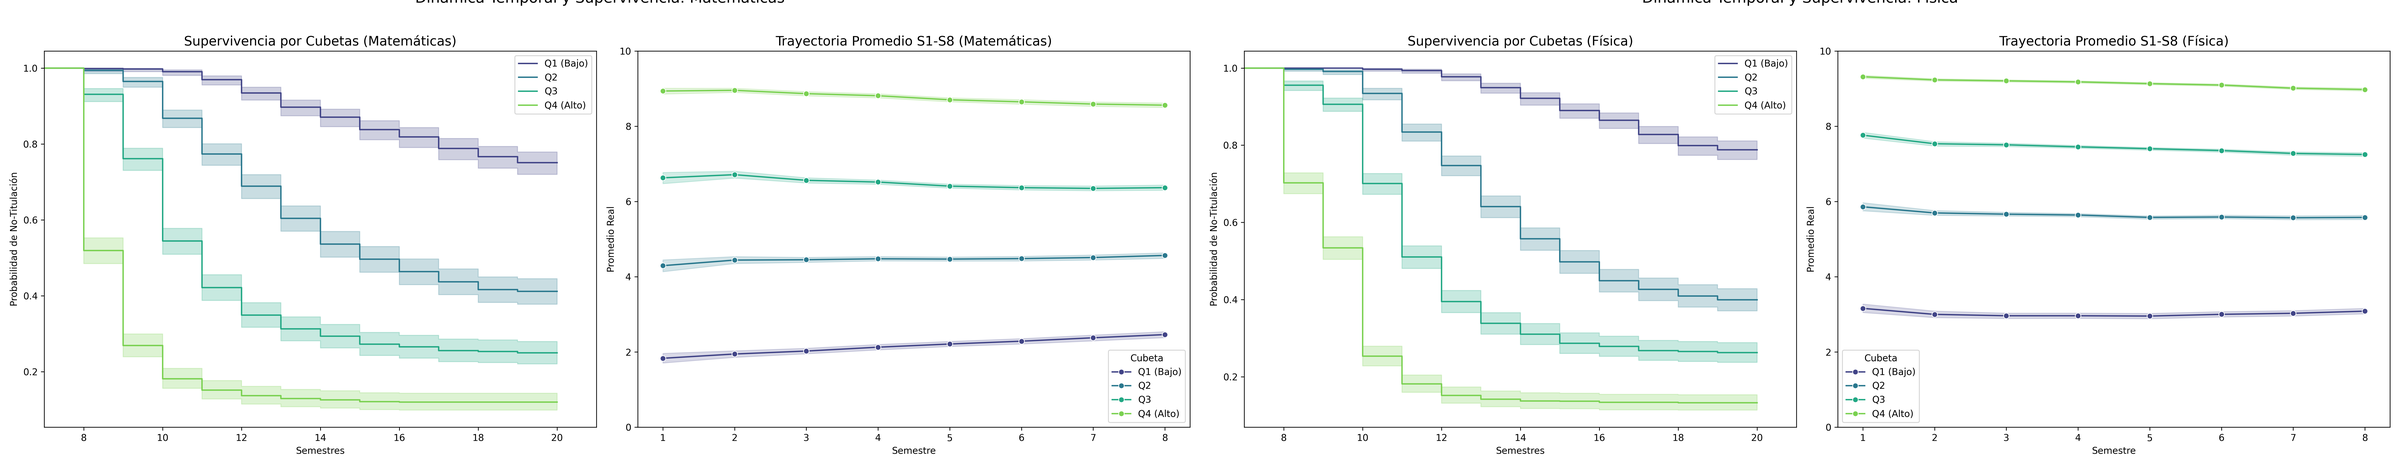
\includegraphics[width=\textwidth]{imagenes/analisis_dual_combined.png}
    \caption{Análisis dual: Supervivencia (izquierda) y Trayectoria de Promedio Real (derecha) para Matemáticas y Física.}
    \label{fig:analisis_dual}
\end{figure}

\section{La Trampa del Perfeccionismo vs. el Pragmatismo}

Uno de los hallazgos más significativos de este estudio es la interacción entre la regularidad y el promedio. Al segmentar a los estudiantes en el cuarto semestre (Tabla \ref{tab:supervivencia_perfiles}), se evidencia que la continuidad administrativa (Regularidad) es un predictor de éxito mucho más potente que la excelencia en la calificación (Promedio Natural).


\begin{table}[H]
\centering
\small
\begin{tabular}{|l|c|c|}
\hline
\textbf{Perfil del Estudiante (al S4)} & \textbf{Mediana Egreso (Mat)} & \textbf{Mediana Egreso (Fis)} \\ \hline
Reg. Alta / Prom. Nat. Alto (Sin atraso) & 10.0 semestres              & 10.0 semestres              \\ \hline
Reg. Alta / Prom. Nat. Bajo (Pragmático) & 11.0 semestres              & 12.0 semestres              \\ \hline
Reg. Baja / Prom. Nat. Alto (Perfeccionista) & $>$ 20 semestres            & $>$ 20 semestres            \\ \hline
Reg. Baja / Prom. Nat. Bajo (Rezago)   & $>$ 20 semestres            & $>$ 20 semestres            \\ \hline
\end{tabular}
\caption{Comparativa de la mediana de tiempo de egreso según el perfil académico al cuarto semestre. Se observa que la Regularidad es el factor determinante: un alumno con promedio bajo pero regularidad alta egresa significativamente antes que uno con promedio alto pero baja regularidad.}
\label{tab:supervivencia_perfiles}
\end{table}

\begin{figure}[H]
    \centering
    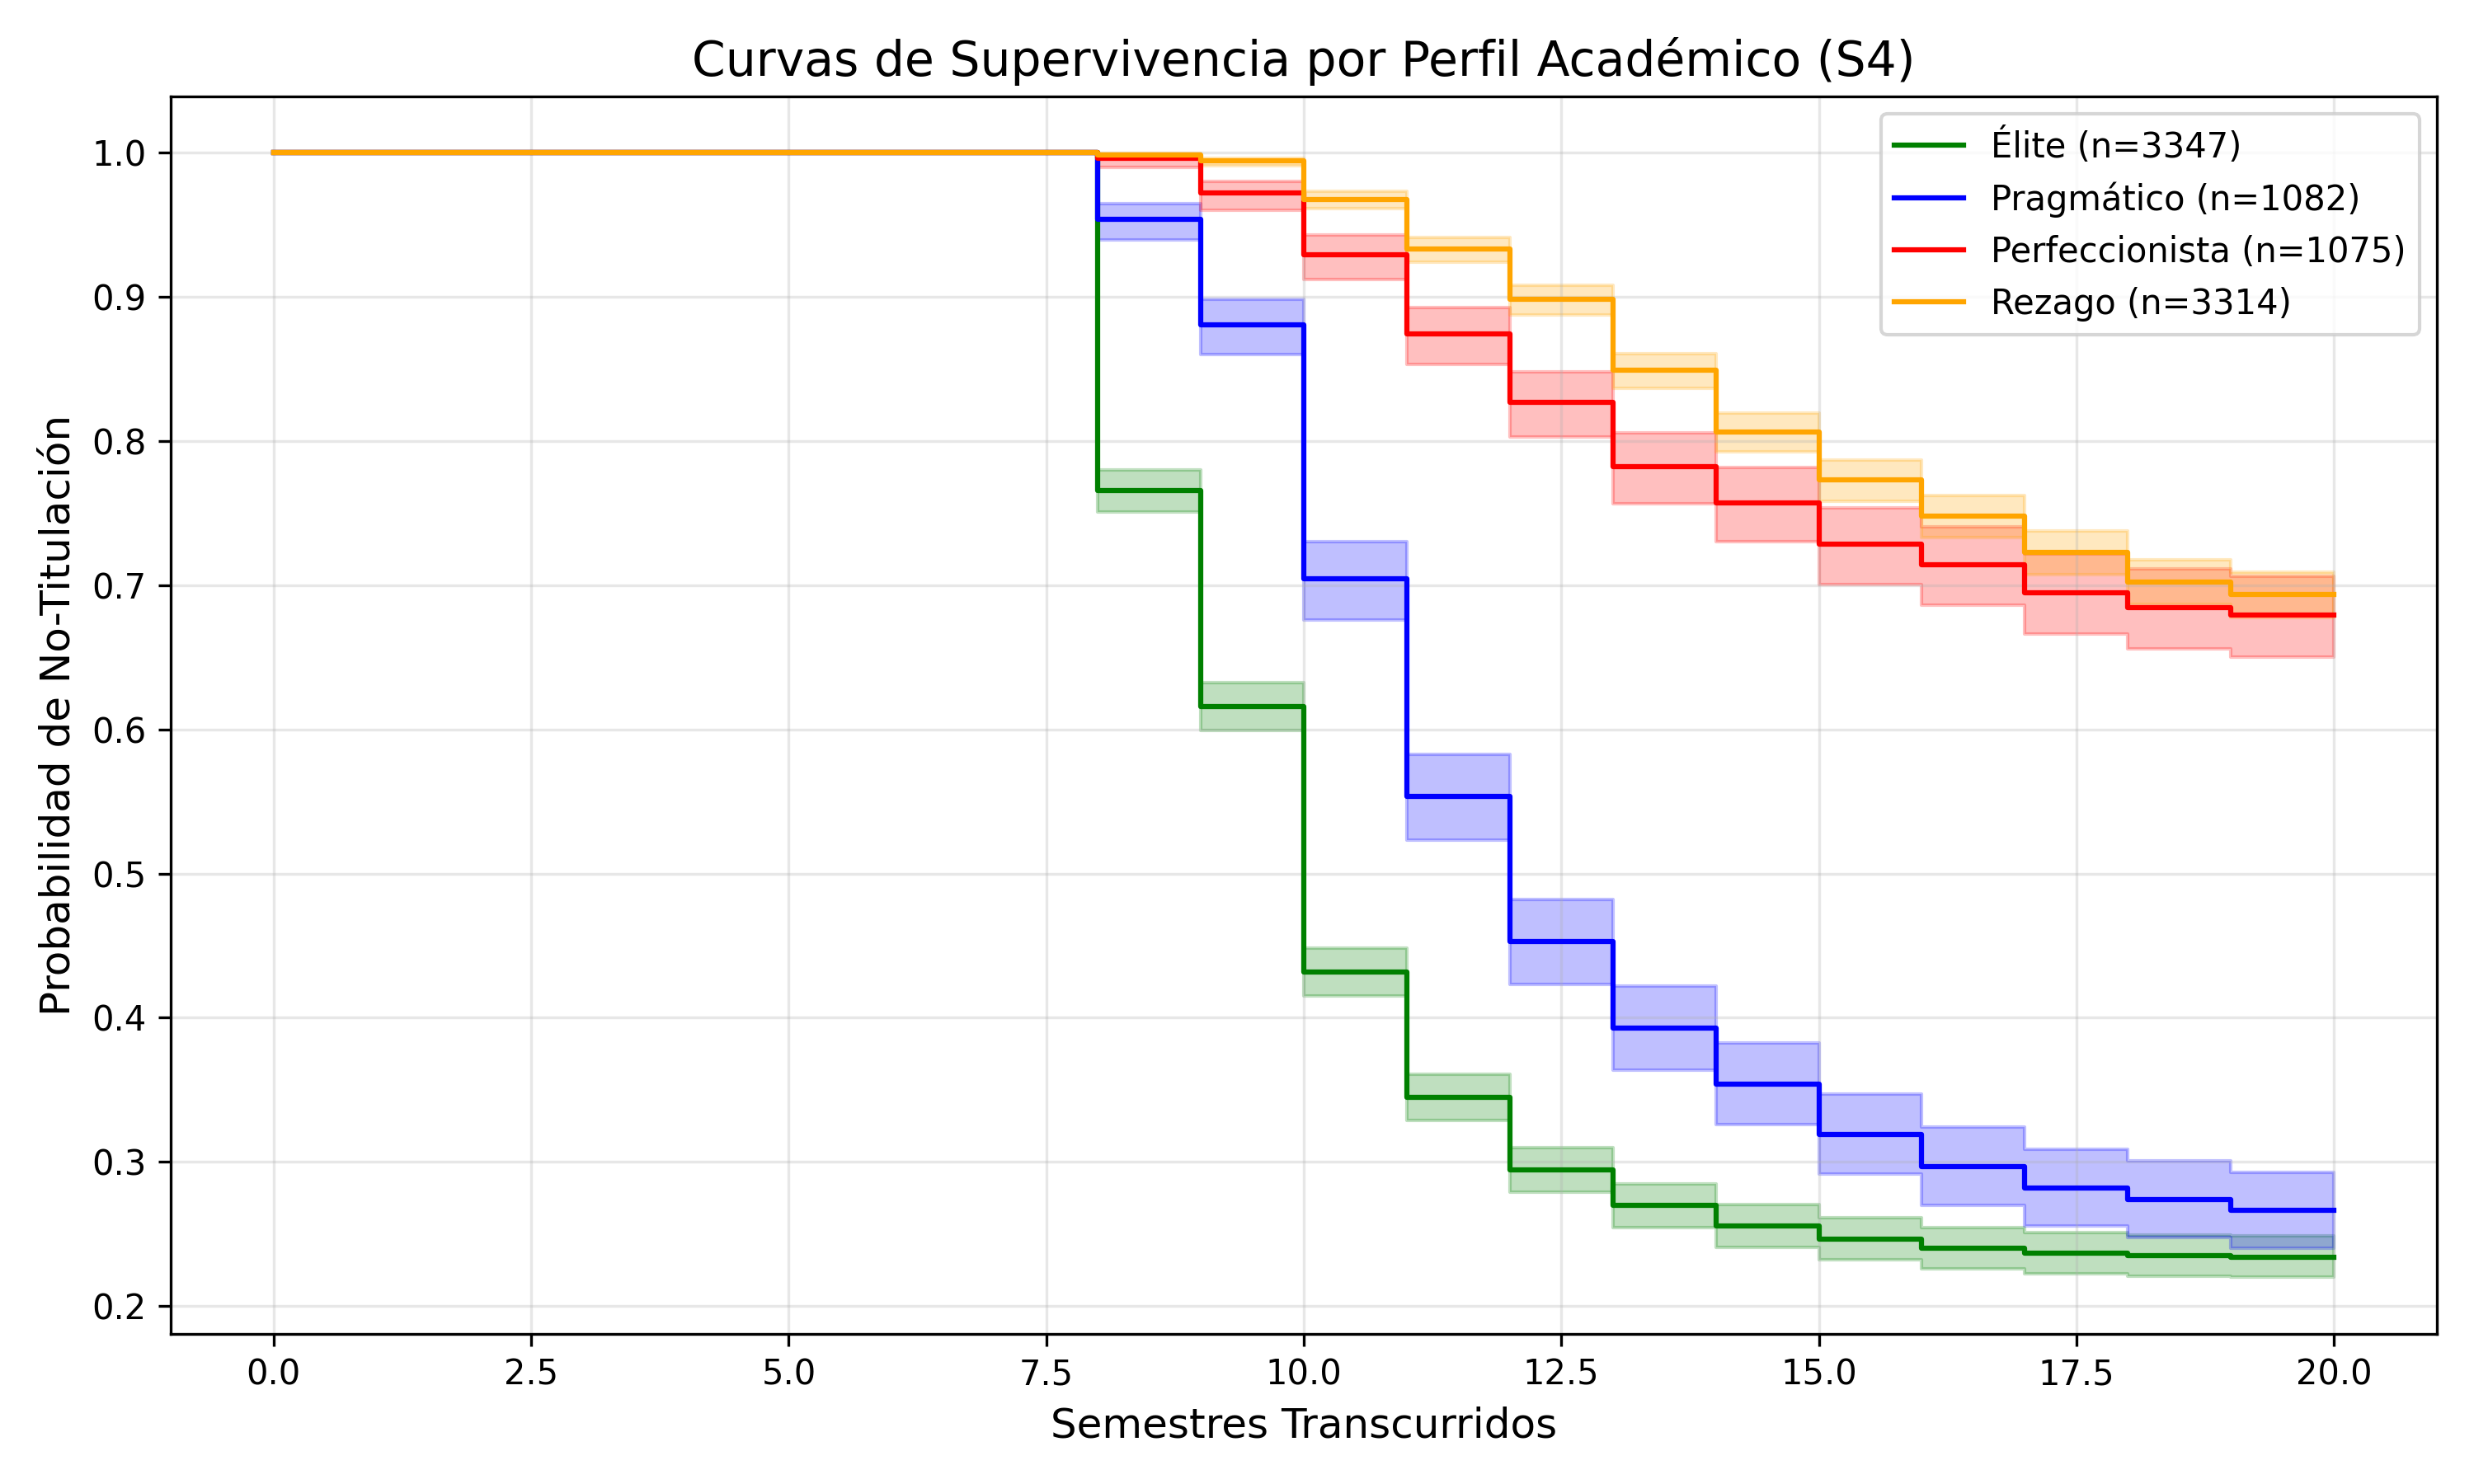
\includegraphics[width=\textwidth]{imagenes/supervivencia_perfiles.png}
    \caption{Curvas de supervivencia de Kaplan-Meier segmentadas por Perfil Académico (S4). Destaca la brecha masiva entre las trayectorias de los estudiantes "Pragmáticos" (azul) y "Perfeccionistas" (rojo).}
    \label{fig:supervivencia_perfiles}
\end{figure}

Este fenómeno sugiere que las estrategias de "sacrificio" de materias para preservar un promedio alto resultan contraproducentes. Para validar estadísticamente esta paradoja, se ajustó un Modelo de Riesgos Proporcionales de Cox utilizando la Regularidad y el Promedio Natural al cuarto semestre como covariables. 

Los resultados confirmaron la dominancia de la regularidad: el \textit{Hazard Ratio} de la regularidad fue de $12.70$ ($p < 0.005$), indicando que es el motor principal del egreso. Sorprendentemente, el efecto del promedio natural no resultó estadísticamente significativo al nivel $\alpha = 0.05$ ($p = 0.08$), desmintiendo la idea de que tener mejores calificaciones acelera el egreso si no se acompaña de ritmo académico. Adicionalmente, una prueba Log-Rank confirmó que las trayectorias de los estudiantes "Pragmáticos" son abismalmente más eficientes que las de los "Perfeccionistas" ($p < 0.0001$), demostrando el daño sistémico de priorizar la calificación sobre la continuidad administrativa.

\section{Estabilidad y Predicción de Largo Plazo}

El análisis de las trayectorias permite identificar patrones de comportamiento que se mantienen constantes a lo largo de la licenciatura. A continuación, se detallan los hallazgos relativos a la estabilidad del desempeño y el impacto de las variables tempranas en el horizonte final de egreso.

\subsection{Inercia Académica y Estabilidad de las Trayectorias}

Se observó una correlación positiva y significativa ($r > 0.60$) entre el promedio real del primer semestre y el desempeño en el octavo semestre para ambas licenciaturas. Este fenómeno, que definiremos como \textit{Inercia Académica}, sugiere una alta estabilidad en las trayectorias: una vez que un estudiante se sitúa en un nivel de rendimiento determinado durante su primer año, la probabilidad de que se desplace hacia otros niveles de desempeño es baja. Esta rigidez refuerza la importancia de las intervenciones pedagógicas y administrativas durante los primeros doce meses de la carrera.

\subsection{Impacto de la Reprobación Temprana en la Regularidad Final}

Al analizar la brecha entre el promedio natural (materias aprobadas) y el promedio real (incluyendo reprobadas) durante el primer semestre, se encontró un vínculo directo con la regularidad de largo plazo. Existe una correlación negativa moderada ($r \approx -0.50$) entre la magnitud de esta brecha inicial y la regularidad en el octavo semestre. Esto indica que el incumplimiento de créditos en la etapa de ingreso no es un evento aislado, sino que actúa como un predictor del rezago administrativo acumulado al final de la carrera.

\subsection{Interacción entre Esfuerzo y Rendimiento al Inicio de la Licenciatura}

Finalmente, se exploró el efecto conjunto del esfuerzo (carga de créditos) y el rendimiento académico. En la licenciatura en Física, el producto del Índice de Esfuerzo por el Promedio Real en el primer semestre resultó ser un predictor del egreso más potente que cualquiera de las dos variables por separado. Este resultado subraya que, en contextos de alta exigencia académica, la capacidad de sostener una carga de trabajo completa manteniendo la calidad en las calificaciones es el factor determinante para asegurar una trayectoria de egreso eficiente.
